\documentclass[a4paper,10pt,DIV=12]{scrreprt}
%\documentclass[a4paper,10pt]{report}
\usepackage{color}
\usepackage[utf8]{inputenc}
\usepackage{graphicx}
\usepackage{verbatim}
\usepackage{hyperref}
\usepackage[usenames,dvipsnames,svgnames,table]{xcolor}
\usepackage[chapter]{minted}
\usemintedstyle{vs}
\renewcommand{\textfraction}{.01}
\hypersetup{
linktoc = all, %linktocpage = true,
colorlinks = true,
linkbordercolor = {white},
linkcolor = {black}}

\newenvironment{code}{%
\center
\minipage{0.9\textwidth}
\hrule\vspace{2mm}
\small
\verbatim
}{%
\endverbatim
\vspace{-1mm}\hrule
\endminipage
\endcenter
}

\newenvironment{shell}{%
\center
\minipage{0.9\textwidth}
\hrule\vspace{2mm}
\small
\verbatim
}{%
\endverbatim
\vspace{-1mm}\hrule
\endminipage
\endcenter
}

% Title Page
\titlehead{%
  \makebox[0pt][l]{\smash{%
    \parbox[t][\dimexpr\textheight-\ht\strutbox\relax][b]{\textwidth}{%
      
\includegraphics[height=0.9in]{images/lbl_logo.png}\hfill
\includegraphics[height=0.9in]{images/cascade_logo.png}%
  }}}}
\title{%\hrule width \hsize height 1pt \vspace{3mm} %
The TECA, Toolkit for Extreme Climate Analysis, User's Guide \\ \vspace{3mm} %
\hrule width \hsize height 1pt \vspace{0.51mm} %
\hrule width \hsize height 1pt}
\subtitle{Lawrence Berkeley National Lab}
\addtocontents{toc}{\protect\hypertarget{toc}{}}

%\author{Burlen Loring, et al.}
\author{}


\begin{document}
\maketitle

% \begin{abstract}
% \end{abstract}

\tableofcontents

\chapter{Installation}
\section{Install the Binary Distribution}
TODO. Jeff has setup the superbuild that we will use to make binaries. The location
from which to download them has not yet been determined. Nor has details like do we use
brew on apple and apt on ubuntu etc.

\section{Build and Install from Sources}
\label{sec:build}
TECA is written in C++11. on Unix like systems
GCC 4.9 or newer, or LLVM 3.5 or newer are required. CMake is needed for configuring the build.
Additionally, TECA relies on a number of third party libraries for various
features and functionality. The dependencies are all optional in the sense
that the build will proceed if they are missing. However, core functionality
may be missing if dependencies are not available. We highly recommend building
TECA with NetCDF, UDUNITS, MPI, Boost, and Python.

\subsection{Installing from Source}
\subsubsection{List of Dependencies}
The full list of dependencies are:

\vspace{2mm}\hspace{0.2in}\begin{minipage}{0.8\textwidth}
\begin{description}
 \item[NetCDF 4:] Required for CF-2.0 file I/O
 \item[HDF5:] Optional, required only for files written in NetCDF 4 HDF5 data format.
 \item[UDUNITS 2:] Required for calendaring
 \item[MPI 3:] Required for MPI parallel operation
 \item[Python, SWIG 3, NumPy:] required for Python bindings
 \item[mpi4py:] Required for parallel Python programming
 \item[Boost:] Required for command line C++ applications
 \item[libxlsxwriter:] Required for binary MS Excel workbook output
\end{description}
\end{minipage}\vspace{2mm}

\subsubsection{Using the TECA\_3rdparty Superbuild} The TECA\_3rdparty package provides
a mechanism for installing TECA and all of the dependencies directly from source. 
This is the recommended approach. To use the superbuild, you will first need to clone
the superbuild repository.

\vspace{2mm}\hspace{0.2in}\begin{minipage}{0.8\textwidth}
\begin{minted}[fontsize=\small]{bash}
#!/bin/bash
git clone https://github.com/LBL-EESA/TECA_3rdparty.git
cd TECA_3rdparty
git submodule update --init --remote
\end{minted}
\end{minipage}\vspace{2mm}

\noindent Then make a build directory, choose an install prefix, choose a platform,
and configure and make.

\vspace{2mm}\hspace{0.2in}\begin{minipage}{0.8\textwidth}
\begin{minted}[fontsize=\small]{bash}
#!/bin/bash
mkdir build && cd build
cmake -DCMAKE_INSTALL_PREFIX=<prefix> \
  -DTECA_PLATFORM=<generic|native> \
  ..
make -j4  && make -j4 install
\end{minted}
\end{minipage}\vspace{2mm}

\noindent In order to make use of the libraries created one
must first configure the environment so that they take precedence over any
conflicting libraries already installed.

\vspace{2mm}\hspace{0.2in}\begin{minipage}{0.8\textwidth}
\begin{minted}[fontsize=\small]{bash}
#!/bin/bash
$ . <prefix>/bin/teca_env.sh
\end{minted}
\end{minipage}\vspace{2mm}

\noindent Note, that the configuration script must be sourced at the start of
each session before using TECA to prevent conflicts with existing installs of
any of the dependencies. This completes the typical TECA install.

\subsection{Installing from a Package Manager}
\textbf{ \color{red} Installing TECA's dependencies via a package manager is not
recommended due to TECA's requirement for a thread safe HDF5 HL library.} If one
does not need support for the NetCDF 4 HDF5 file format then installing from a
package manager is a viable option.

\subsubsection{Using apt on Ubuntu 14.04}
The following shows how to install dependencies on Ubuntu 14.04:

\vspace{2mm}\hspace{0.2in}\begin{minipage}{0.8\textwidth}
\begin{minted}[fontsize=\small]{bash}
#!/bin/bash
# setup repo with recent package versions
sudo add-apt-repository -y ppa:ubuntu-toolchain-r/test
sudo add-apt-repository -y ppa:teward/swig3.0
sudo apt-get update -qq
# install deps
sudo apt-get install -qq -y cmake gcc-5 g++-5 gfortran swig3.0 \
    libopenmpi-dev openmpi-bin libhdf5-openmpi-dev libnetcdf-dev \
    libboost-program-options-dev python-dev libudunits2-0 \
    libudunits2-dev
# use PIP for Python packages
pip install --user numpy mpi4py
\end{minted}
\end{minipage}\vspace{2mm}

\noindent Note that on more recent releases of Ubuntu one will not need to use PPA repos to obtain up to date packages.
Other Linux distros, such as Fedora, have a similar install procedure albeit with different package names.
\textbf{\color{red} The apt install does not provide threadsafe HDF5! If your data is in NetCDF 4 HDF5 format please use the
TECA\_3rdparty superbuild}.

\subsubsection{Using brew on Apple Mac OSX Yosemite}
On Apple Mac OSX using homebrew to install the dependencies is recommended.

\vspace{2mm}\hspace{0.2in}\begin{minipage}{0.8\textwidth}
\begin{minted}[fontsize=\small]{bash}
#!/bin/bash
brew update
brew tap Homebrew/homebrew-science
brew install gcc openmpi hdf5 netcdf python swig udunits
brew install boost --C++11
pip install numpy mpi4py
\end{minted}
\end{minipage}\vspace{2mm}

\noindent We highly recommend taking a look a the output of \textbf{brew doctor} and
fixing all reported issues before attempting a TECA build. Significant
complications can arise where user's have mixed installation methods, such as mixing
installs from macports, homebrew, or manual installs. Multiple Python installations
can also be problematic. During configuration TECA reports the Python version detected,
one should verify that this is correct and if not set the paths manually. \textbf{
\color{red} The brew install does not provide threadsafe HDF5! If your data is in
NetCDF 4 HDF5 format please use the TECA\_3rdparty superbuild}.

\subsubsection{Installing TECA}
Once the dependencies have been installed TECA may be compiled and installed. Note,
the TECA\_3rdparty superbuild will build and install TECA by default. This section
is targeted toward those installing dependencies via a package manager or developers
who need a build that is not installed.

\paragraph{Obtaining the Sources} To obtain the TECA sources, clone our github repository.

\vspace{2mm}\hspace{0.2in}\begin{minipage}{0.8\textwidth}
\begin{minted}[fontsize=\small]{bash}
git clone git@github.com:LBL-EESA/TECA.git
\end{minted}
\end{minipage}\vspace{2mm}

\noindent TECA comes with a suite of regression tests. If you wish to validate your build,
you'll also need to obtain the test datasets.

\vspace{2mm}\hspace{0.2in}\begin{minipage}{0.8\textwidth}
\begin{minted}[fontsize=\small]{bash}
svn co svn://missmarple.lbl.gov/work3/teca/TECA_data
\end{minted}
\end{minipage}\vspace{2mm}

\noindent Before compiling you'll need to install the dependencies. See the following sections
for operating system specific instructions.

\paragraph{Compiling TECA} Once dependencies are installed a TECA build can be configured and compiled. The
following sections show operating specific examples of compiling TECA.
TECA\_SOURCE\_DIR should be replaced with the path to the TECA sources,
TECA\_DATA\_DIR replaced with the path to the test data, and TECA\_INSTALL\_DIR
replaced with the path to the install location. \\

\noindent Note that on all operating systems TECA requires an out of source build. The first step is
to create a build directory and cd into it.

\vspace{2mm}\hspace{0.2in}\begin{minipage}{0.8\textwidth}
\begin{minted}[fontsize=\small]{bash}
#!/bin/bash
mkdir ${TECA_SOURCE_DIR}/build
cd ${TECA_SOURCE_DIR}/build
\end{minted}
\end{minipage}\vspace{2mm}

\paragraph{Ubuntu 14.04} $\;$ \\ \\
\vspace{0mm}\hspace{0.2in}\begin{minipage}{0.8\textwidth}
\begin{minted}[fontsize=\small]{bash}
#!/bin/bash
cmake \
    -DCMAKE_C_COMPILER=`which gcc-5` \
    -DCMAKE_CXX_COMPILER=`which g++-5` \
    -Dswig_cmd=`which swig3.0` \
    -DCMAKE_BUILD_TYPE=Release \
    -DCMAKE_INSTALL_PREFIX=${TECA_INSTALL_DIR} \
    -DBUILD_TESTING=ON \
    -DTECA_DATA_ROOT=${TECA_DATA_DIR} \
    ${TECA_SOURCE_DIR}

make -j4 && make -j4 install
\end{minted}
\end{minipage}\vspace{2mm}

\noindent Here compilers and swig are explicitly set to prevent the older and not fully C++11
compliant versions present on Ubuntu 14.04 from being used. On newer releases and other distros
this is not necessary.

\paragraph{Apple Mac OSX Yosemite} $\;$ \\ \\
\vspace{0mm}\hspace{0.2in}\begin{minipage}{0.8\textwidth}
\begin{minted}[fontsize=\small]{bash}
#!/bin/bash
cmake \
    -DCMAKE_BUILD_TYPE=Release \
    -DCMAKE_INSTALL_PREFIX=${TECA_INSTALL_DIR} \
    -DBUILD_TESTING=ON \
    -DTECA_DATA_ROOT=${TECA_DATA_DIR} \
    ${TECA_SOURCE_DIR}

make -j4 && make -j4 install
\end{minted}
\end{minipage}\vspace{2mm}
% \subsubsection{Cray XC 40}
%
% \vspace{2mm}\hspace{0.2in}\begin{minipage}{0.8\textwidth}
% \begin{minted}[fontsize=\small]{bash}
%
% \end{minted}
% \end{minipage}\vspace{2mm}

\subsubsection{Configuring the Environment}
Depending on your configuration PATH and LD\_LIBRARY\_PATH (or DYLD\_LIBRARY\_PATH on Apple)
may need to include your TECA\_INSTALL\_DIR. Additionally,
use of TECA's Python modules require setting PYTHONPATH. Note that the superbuild includes
a script to configure the environment. The following is only necessary when not using
TECA installed via the superbuild.

\paragraph{Ununtu 14.04} $\;$ \\ \\
\vspace{2mm}\hspace{0.2in}\begin{minipage}{0.8\textwidth}
\begin{minted}[fontsize=\small]{bash}
#!/bin/bash
export PATH=${TECA_INSTALL_DIR}/bin:.:$PATH
export PYTHONPATH=${TECA_INSTALL_DIR}/lib:$PYTHONPATH
export LD_LIBRARY_PATH=${TECA_INSTALL_DIR}/lib:$LD_LIBRARY_PATH
\end{minted}
\end{minipage}\vspace{2mm}

\paragraph{Apple Mac OSX Yosemite} $\;$ \\ \\
\vspace{2mm}\hspace{0.2in}\begin{minipage}{0.8\textwidth}
\begin{minted}[fontsize=\small]{bash}
#!/bin/bash
export PATH=${TECA_INSTALL_DIR}/bin:.:$PATH
export PYTHONPATH=${TECA_INSTALL_DIR}/lib:$PYTHONPATH
export LD_LIBRARY_PATH=${TECA_INSTALL_DIR}/lib:$LD_LIBRARY_PATH
export DYLD_LIBRARY_PATH=${TECA_INSTALL_DIR}/lib:$DYLD_LIBRARY_PATH
\end{minted}
\end{minipage}\vspace{2mm}



\subsection{Validating the Install}
TECA comes with an extensive regression test suite which can be used to validate
your build. The tests can be executed from the build directory with the ctest command.

\vspace{2mm}\hspace{0.2in}\begin{minipage}{0.8\textwidth}
\begin{minted}[fontsize=\small]{bash}
#!/bin/bash
ctest --output-on-failure
\end{minted}
\end{minipage}\vspace{2mm}

\noindent Do not forget to configure the environment as described above.

% \subsection{TECA}
% \label{sec:build}
% \paragraph{Supported Compilers}
% Building TECA requires a C++1111 compiler. On Unix like systems this is GCC
% 4.9(or newer), or LLVM 3.5(or newer). Windows MS Visual Studio C++11 currently
% does not fully support C++1111. The following dependencies are optional, however
% functionality will be reduced if they are not present.
%
% \begin{itemize}
% \item CMake for configuring the build
% \item NetCDF for the CF reader
% \item MPI for distributed parallel operation
% \item Boost program\_options for the command line applications
% \item VTK for the ability to save mesh based data for later visualization in ParaView or VisIt
% \end{itemize}
%
% The location of various dependencies should be passed
% in during configuration if they are in non-standard locations. It's is critical
% that compiler and C++11 library versions match across dependencies, especially Boost.
%
% \paragraph{Compiling TECA on a Workstation}
% This is an example of compiling on a work station, with Boost, MPI, NetCDF and
% VTK features enabled:
% \begin{code}
#!/bin/bash 

cmake \
    -DCMAKE_CXX_COMPILER=`which clang++` \
    -DCMAKE_C_COMPILER=`which clang` \
    -DCMAKE_BUILD_TYPE=Release \
    -DNETCDF_DIR=/work/apps/netcdf/4.3.3.1/ \
    -DVTK_DIR=/work/apps/vtk/next/lib/vtk-6.3/cmake \
    -DBOOST_ROOT=/work/apps/boost/1.58.0 \
    $*

make -j8 && make -j8 install
\end{code}

\paragraph{Compiling TECA on a Cray}
The following shows how TECA is compiled on NERSCs Cray XC30 Edison with Boost,
MPI, and NetCDF.

\begin{code}
#!/bin/bash

module load cmake/3.0.0
module swap PrgEnv-intel PrgEnv-gnu
module load netcdf/4.3.3.1
module load boost/1.58.0

export XTPE_LINK_TYPE=dynamic
LIB_EXT=so

NETCDF=/usr/common/graphics/netcdf/4.3.3.1
BOOST=/usr/common/graphics/boost/1.58.0/

SMA=/opt/cray/mpt/7.2.1/gni/sma/lib64
MPT=/opt/cray/mpt/7.2.1/gni/mpich2-gnu/49/lib
RCA=/opt/cray/rca/1.0.0-2.0502.57212.2.56.ari/lib64
ALPS=/opt/cray/alps/5.2.3-2.0502.9295.14.14.ari/lib64
XPMEM=/opt/cray/xpmem/0.1-2.0502.57015.1.15.ari/lib64
DMAPP=/opt/cray/dmapp/7.0.1-1.0502.10246.8.47.ari/lib64
PMI=/opt/cray/pmi/5.0.6-1.0000.10439.140.2.ari/lib64
UGNI=/opt/cray/ugni/6.0-1.0502.10245.9.9.ari/lib64
UDREG=/opt/cray/udreg/2.3.2-1.0502.9889.2.20.ari/lib64
WLM=/opt/cray/wlm_detect/1.0-1.0502.57063.1.1.ari/lib64
ATP=/opt/cray/atp/1.8.2/libApp

CXXCOMP=`which g++`
CCOMP=`which gcc`

cmake \
  -DCMAKE_CXX_COMPILER=$CXXCOMP \
  -DCMAKE_C_COMPILER=$CCOMP \
  -DCMAKE_BUILD_TYPE=Release \
  -DCMAKE_EXE_LINKER_FLAGS_RELWITHDEBINFO="$ATP/libAtpSigHandler.$LIB_EXT $ATP/libAtpSigHCommData.a -Wl,--undefined=_ATP_Data_Globals -Wl,--undefined=__atpHandlerInstall" \
  -DCMAKE_EXE_LINKER_FLAGS_DEBUG="$ATP/libAtpSigHandler.$LIB_EXT $ATP/libAtpSigHCommData.a -Wl,--undefined=_ATP_Data_Globals -Wl,--undefined=__atpHandlerInstall" \
  -DMPI_CXX_COMPILER=$CXXCOMP \
  -DMPI_C_COMPILER=$CCOMP \
  -DMPI_CXX_LIBRARIES="" \
  -DMPI_C_LIBRARIES="-Wl,--start-group;$MPT/libmpichcxx.$LIB_EXT;$SMA/libsma.$LIB_EXT;$PMI/libpmi.$LIB_EXT;$DMAPP/libdmapp.$LIB_EXT;$MPT/libmpichcxx_gnu_49.$LIB_EXT;$UGNI/libugni.$LIB_EXT;$ALPS/libalpslli.$LIB_EXT;$WLM/libwlm_detect.$LIB_EXT;$ALPS/libalpsutil.$LIB_EXT;$RCA/librca.$LIB_EXT;$XPMEM/libxpmem.$LIB_EXT;-Wl,--end-group;" \
  -DMPI_INCLUDE_PATH=$MPT/../include \
  -DMPIEXEC=$APRUN/bin/aprun \
  -DNETCDF_DIR=$NETCDF \
  -DBOOST_ROOT=$BOOST \
  -DCMAKE_INSTALL_PREFIX=/usr/common/graphics/teca/1.0 \
  ../teca

make -j 8 && make -j 8 install
\end{code}
%
% \subsection{Prerequisites}
% Dependencies can be installed from a package manager where convenient. However,
% note that particularly with Boost, compiler and stdlib used to build Boost must
% match that used with TECA. When using cmake on systems with multiple compilers
% one must consistently specify CMAKE\_CXX\_COMPILER and CMAKE\_C\_COMPILER and/or
% export CC and CXX environment variables.
%
% \paragraph{CMake}
% TECA builds are configured with CMake. Version 2.8.12 or newere is required.
% Installing via your system's package manager is recommended.
%
% \paragraph{MPI}
% MPI is required for distributed parallel operation. It's recommended to use
% the package management system on your OS to install MPI.
%
% \paragraph{NetCDF}
% A standard make, make install suffices. It is fine to disable NetCDF 4 features. Replace
% gcc and g++ with your compiler, for example clang and clang++ on Apple.
%
% \begin{code}
% export CC=`which gcc`
% export CXX=`which g++`
% wget ftp://ftp.unidata.ucar.edu/pub/netcdf/netcdf-4.3.3.1.tar.gz
% tar xzfv netcdf-4.3.3.1.tar.gz
% cd netcdf-4.3.3.1
% ./configure --disable-netcdf-4 --prefix=/work/apps/netcdf/4.3.3.1
% make -j2 && make -j4 install
% \end{code}
%
% \paragraph{Boost}
% When possible use the package manager to install Boost. However note that the
% compiler and stdlib version used to build Boost **needs to match exactly** the
% compiler and stdlib used to build TECA. This may necessitate a stand alone
% Boost install.
%
% On Linux if the compiler yo are using is in the PATH then a simple install
% suffices.
% boost_link="http://downloads.sourceforge.net/project/boost/boost/1.58.0/boost_1_58_0.tar.gz?r=http%3A%2F%2Fsourceforge.net%2Fprojects%2Fboost%2Ffiles%2Fboost%2F1.58.0%2F&ts=1434648565&use_mirror=tcpdiag"
% \begin{code}
% #!/bin/bash
% curl -L <HTTP LINK TO BOOST PACKAGE> -o boost.tar.gz
% tar xzfv boost.tar.gz
% cd boost_1_58_0/
% ./bootstrap.sh --prefix=/Users/bloring/apps/
% ./b2 -j4 cxxflags=''-std=C++11'' install
% \end{code}
%
% However, on Apple, when using clang you must specify toolset and flags when
% building Boost:
%
% \begin{code}
% #!/bin/bash
% ./b2 -j4 toolset=clang cxxflags="-stdlib=libC++" linkflags="-stdlib=libC++" install
% \end{code}
%
% \paragraph{Python}
% TECA's Python bindings are enabled by setting the CMake variable TECA\_PYTHON\_BINDING=ON during configuration. The Python bindings may be compiled without SWIG. However, SWIG must be installed for TECA development work.
% notes for debug
% if you see the following when you import
% teca modules then you are mixing two or more
% Python installs
%
% Fatal Python error: PyThreadState\_Get: no current thread
% Abort trap: 6
%
% you must use shared libraries on Mac OSX with Python. Linux seems to be OK.
% SWIG documentation warns about this.
%
% \paragraph{VTK}
% \begin{code}
% #!/bin/bash
% git clone git://VTK.org/VTK.git
% mkdir vtk_build
% cd vtk_build
% cmake \
%   -DCMAKE_CXX_COMPILER=`which g++` \
%   -DCMAKE_C_COMPILER=`which gcc` \
%   -DCMAKE_INSTALL_PREFIX=/work/apps/VTK/next \
%   ../VTK
% make -j4 && make -j4 install
% \end{code}
%
% \section{Running the Pre-packaged Applications}
% See --help and --full\_help command line arguments for the application in question.
%
% \subsection{AR Detector}
% \paragraph{Running on a Cray}
% make a qsub file and submit a job. Here is an example:
% \begin{code}
% #!/bin/bash -l
% #PBS -q premium
% #PBS -l mppwidth=2400
% #PBS -l walltime=01:00:00
% #PBS -N teca_tmq
% #PBS -j oe
%
% TECA_HOME=/usr/common/graphics/teca/1.0
%
% cd $PBS_O_WORKDIR
% aprun -n 200 -N 2 -S 1 \
%     ${TECA_HOME}/bin/teca_ar_detect \
%         --water_vapor_file_regex TMQ_cam5_1_amip_run2'.*nc' \
%         --water_vapor_var TMQ \
%         --n_threads 12 \
%         --results_file tmq_ar.csv
% \end{code}
%
% \subsection{TC Detector}
% \subsection{ETC Detector}
% \chapter{The TECA Libraries}
% \label{sec:lib}
% \section{Input and Data Readers}
% \section{Detectors}
% \section{Analsyis}
% \section{Re-meshing}
% \section{Output and Data Writers}
\chapter{Tropical Cylone Detector}
\section{NERSC}
Once on Edison load the TECA module
\begin{minted}{bash}
module load teca
\end{minted}
note that there are multiple versions installed, just use the latest and greatest as they become available.

Processing an entire dataset is straight forward once you know how many cores you want to run on. You will launch teca\_tc\_detect, the tropical cyclone application, from a SLURM batch script. A batch script is provided below. The most common options are:
\begin{description}
\item[--help] prints documentation for the most common options. MPI programs, such as teca\_tc\_detect aren't allowed to run on the login noes at NERSC. For this reason to use \textit{--help} you'll need to obtain a compute node via \textit{salloc} first.
\item[--full\_help] prints documentation for all options. See \textit{--help} notes.
\item[--input\_regex]this is how you tell TECA what files are in the dataset. We use the grep style regex, which must be quoted with single ticks to protect it from the shell. Regex meta characters present in the file name must be escaped with a \textbackslash. An example of an input regex which includes all .nc files is: '.*\textbackslash.nc\$'. If instead one wanted to grab only files from 2004-2005 then '.*\textbackslash.200[45].*\textbackslash.nc\$' would do the trick. For the best performance, specify the smallest set of files needed to achieve the desired result. Each of the files will be opened in order to scan the time axis.
\item[--start\_date], an optional way to further specify the time range to process. The accepted format is a CF style human readable date spec such as YYYY-MM-DD hh:mm:ss. Because of the space in between day and hour spec quotes must be used. For example "2005-01-01 00:00:00". Specifying a start date is optional,  if none is given then all of the time steps in all of the files specified in the \textit{--input\_regex} are processed.
\item[--end\_date] see \textit{--start\_date}. this is has a similar purpose in restricting the range of time steps processed.
\item[--candidate\_file], a file name specifying where to write the storm candidates to. If not specified result will be written to candidates.bin in the current working directory. One sets the output format via the extension. Supported formats include csv, xlsx, and bin.
\item[--track\_file], a file name specifying where to write the detected storm tracks. If not specified the tracks are written to a file named tracks.bin in the current working directory. See \textit{--candidate\_file} for information about the supported formats.
\end{description}

TECA can process any size dataset on any number of compute cores. However, the fastest results are attained when there is 1 time step per core. In order to set this up one must determine how many time steps there are and write the SLURM batch script accordingly. The teca\_metadata\_probe command line application can be used for this purpose. When executed with the same \textit{--input\_regex} and optionally the \textit{--start\_date} and or \textit{--end\_date} options that will be used in the cyclone detection run it will print out the information needed to configure a 1 to 1 (time steps to cores) run. The metadata probe is a serial application and can be run on the login nodes.

\begin{minted}{bash}
teca_metadata_probe --input_regex '.*\.199[0-9].*\.nc$'

# A total of 29200 steps available in 3650 files. Using the noleap calendar.
# Times are specified in units of days since 1979-01-01 00:00:00. The available
# times range from 1990-1-1 3:0:0 (4015.12) to 2000-1-1 0:0:0 (7665).
\end{minted}

With the number of time steps in hand one can set up the SLURM batch script for the run. The following batch script, named \textit{1990s.sh}, processes the entire decade of the 1990's. The teca\_metadata\_probe was used to determine that there are 29200 time steps. The srun command is used to launch the cyclone detector on 29200 cores.
\begin{minted}{bash}
#!/bin/bash -l

#SBATCH -p regular
#SBATCH -N 1217
#SBATCH -t 00:30:00

data_dir=/scratch2/scratchdirs/prabhat/TCHero/data
files_regex=cam5_1_amip_run2'\.cam2\.h2\.199[0-9].*.nc$'

srun -n 29200 teca_tc_detect                    \
    --input_regex ${data_dir}/${files_regex}    \
    --candidate_file candidates_1990s.bin       \
    --track_file tracks_1990s.xlsx
\end{minted}
Finally, the batch script must be submitted to the batch system requesting the appropriate number of nodes. In this case the command is:
\begin{minted}{bash}
$sbatch ./1990s.sh
\end{minted}

For the $\frac{1}{4}$ degree resolution dataset when processing latitudes between -90 to 90 the detctor runs in approx 15min. Detector run time could be reduced by subsetting in latitude (see \textit{--lowest\_lat}, \textit{--highest\_lat} options). Note that as the number of files in the dataset increases the metadata phase takes more time. You can use teca\_metadata\_probe to get a sense of how much more and extend the run time accordingly.

\chapter{Python}
TECA includes a diverse collection of I/O and analysis algorithms specific to climate science and extreme event detection. It's pipeline design allows these component algorithms to be quickly coupled together to construct complex data processing and analysis pipelines with minimal effort. TECA is written primarily in C++11 in order to deliver the highest possible performance and scalability. However, for non-computer scientists c+11 development can be intimidating, error prone, and time consuming. TECA's Python bindings offer a more approachable path for custom application and algorithm development.

Python can be viewed as glue for connecting optimized C++11 components. Using Python as glue gives one all of the convenience and flexibility of Python scripting with all of the performance of the native C++11 code. TECA also includes a path for fully Python based algorithm development where the programmer provides Python callables that implement the desired analysis. In this scenario the use of technologies such as NumPy provide reasonable performance while allowing the programmer to focus on the algorithm itself rather than the technical details of C++11 development.

\begin{figure}[h]
 \centering
 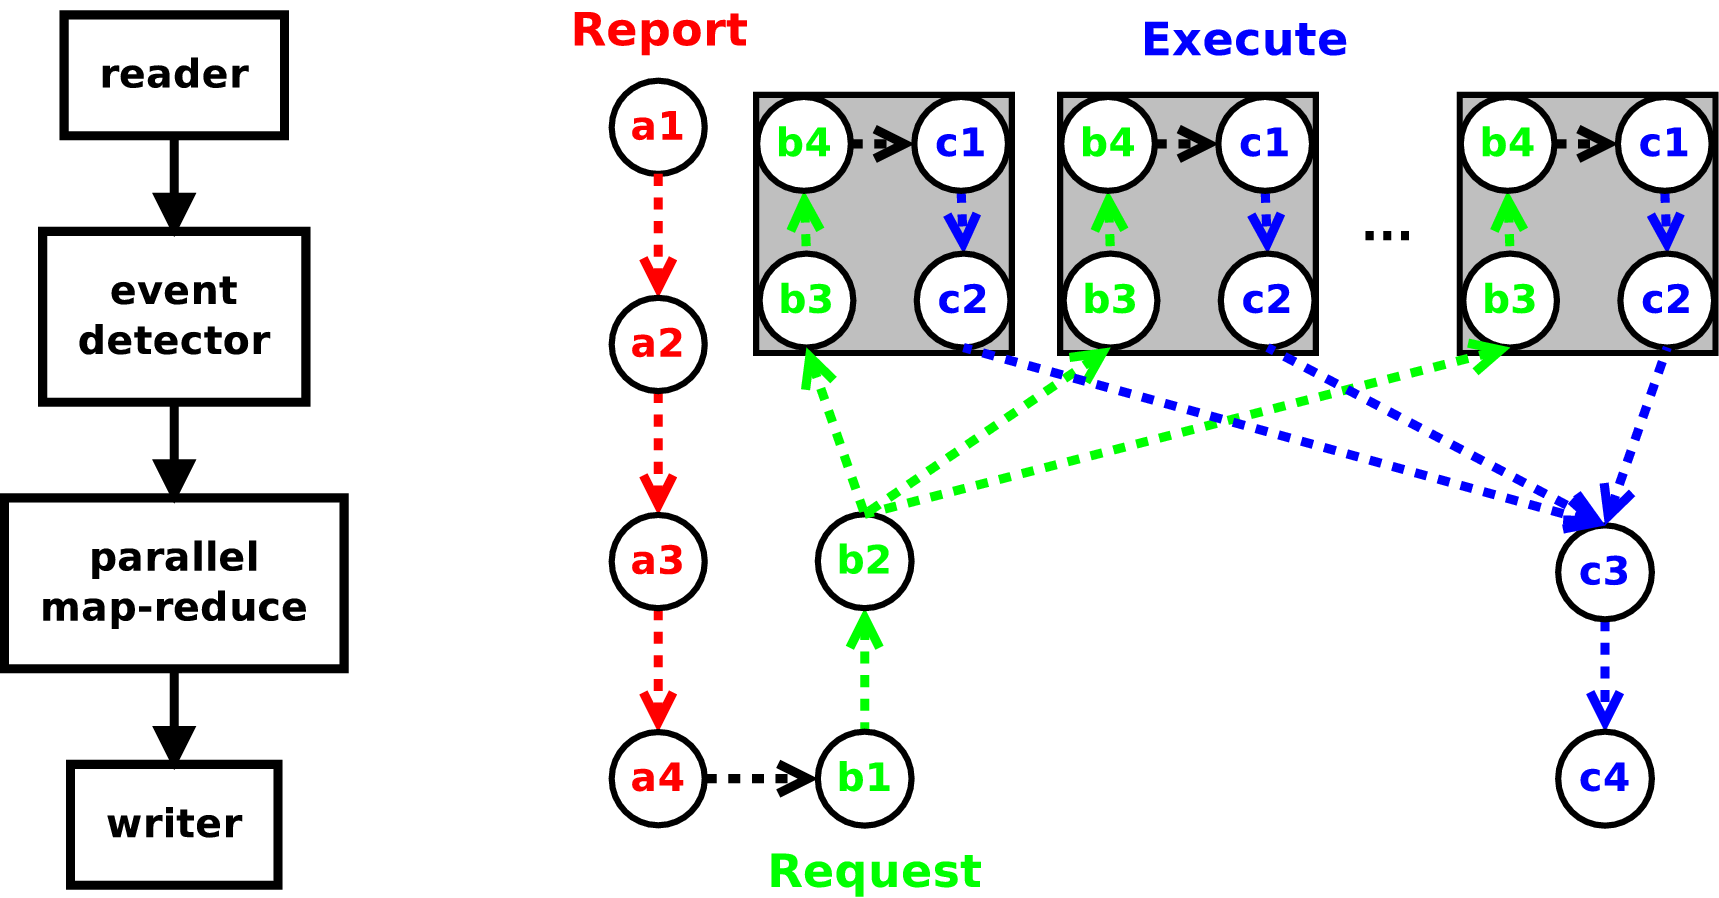
\includegraphics[height=2.5in]{./images/parallel_exec.png}
 % serial_exec.png: 0x0 pixel, 300dpi, 0.00x0.00 cm, bb=
 \caption{\small  execution path through a simple 4 stage pipeline on any given process in an MPI parallel run. Time progresses from a1 to c4 through the three execution phases report (a), request (b), and execute (c). The sequence of thread parallel execution is shown inside gray boxes, each path represents the processing of a single request.}
 \label{fig:parallel_exec}
\end{figure}

\section{Pipeline Construction, Configuration and Execution}
\label{sec:py_glue}
Building pipelines in TECA is as simple as creating and connecting TECA algorithms together in the desired order. Data will flow and be processed sequentially from the top of the pipeline to the bottom, and in parallel where parallel algorithms are used. All algorithms are created by their static New() method. The connections between algorithms are made by calling one algorithm's set\_input\_connection() method with the return of another algorithm's get\_output\_port() method. Arbitrarily branchy pipelines are supported. The only limitation on pipeline complexity is that cycles are not allowed. Each algorithm represents a stage in the pipeline and has a set of properties that configure its run time behavior. Properties are accessed by set\_<prop name>\(\) and get\_<prop name>\(\) methods. Once a pipeline is created and configured it can be run by calling update() on its last algorithm.

\begin{listing}[h]
\begin{center}
\vspace{1mm}
\begin{minipage}{0.8\textwidth}
\inputminted[fontsize=\footnotesize, linenos]{python}{source/stats.py}
\caption{\small Command line application written in Python. The application constructs, configures, and executes a 4 stage pipeline that computes basic descriptive statistics over the entire lat-lon mesh for a set of variables passed on the command line. The statistic computations have been written in Python, and are shown in listing \ref{code:py_devel}. When run in parallel, the map-reduce pattern is applied over the time steps in the input dataset. A graphical representation of the pipeline is shown in figure \ref{fig:parallel_exec}.}
\label{code:py_glue}
\end{minipage}
\end{center}
\end{listing}

For example, listing \ref{code:py_glue} shows a command line application written in Python. The application computes a set of descriptive statistics over a list of arrays for each time step in the dataset. The results at each time step are stored in a row of a table. teca\_table\_reduce is a map-reduce implementation that processes time steps in parallel and reduces the the tables produced at each time step into a single result. One use potential use of this code would be to compute a time series of average global temperature. The application loads modules and initializes MPI (lines 1-6), parses the command line options (lines 8-19),  constructs and configures the pipeline (lines 24-40), and finally executes the pipeline (line 42). The pipeline constructed is shown in figure \ref{fig:parallel_exec} next to a time line of the pipeline's parallel execution on an arbitrary MPI process.

% \paragraph{Execution and Parallelism}
% Once a pipeline has been built and configured it is executed by calling update() on one of the algorithms. Typically, update is called on the last algorithm in the pipeline. Line 51 in listing \ref{code:py_glue} executes the example pipeline. \mint{python}|twr.upadte()| TECA's pipeline model uses ``requests'' to pull only the data that is needed through the pipeline on demand. Requests enable streaming of data and can be acted upon in parallel. Also requests are used as a key in the pipeline's internal cache. Thus requests play a very important role in TECA's execution model. Simple data processing algorithms should not include request generation logic. Instead copy, modify, and forward the incoming request. This ensures that details of the request are not lost as it travels upstream.

% Algorithms that partition work amongst processes and threads need to implement request generation logic. For instance teca\_temporal\_reduction and the classes derived from it. teca\_temporal\_reduction is an abstract class that implements parallel map-reduce over time steps. The abstract class teca\_temporal\_reduction generates a request per time step and parallelizes request execution using MPI and threads. The generated requests are first partitioned to MPI processes and within MPI processes a threadpool processes the local requests. teca\_temporal\_reduction handles all of the inter-process communication needed to complete the reduction. It's parent class teca\_threaded\_algorithm manages the thread pool and putting requests into its work queue and getting data back out. Classes derived from teca\_temporal\_reduction provide the data type specific code. For example, teca\_table\_reduce implements map-reduce over tabular data. There are a few things to keep in mind when using one of TECA's map-reduce classes. To make your program parallel simply initialize MPI. \mint{python}|from mpi4py import MPI| Everything above the map-reduce class is executed in parallel. Everything below is executed in serial on MPI rank 0. Finally one need not worry about source of requests when using TECA's map-reduce this is handled internally.
%
% When not using one of TECA's map-reduce implementations one must explicitly proivide a request generator to the algorithm upon which update() is called. In TECA request generater is call an \emph{executive}. The most common use case is to generate a request per time step. This is the purpose of the teca\_time\_step\_executive. It's use is demonstrated in listing \ref{code:py_devel} lines 43-45. Keep in mind that the teca\_time\_step\_executive is not MPI or thread aware, and should not be used for parallel programs.
% \begin{minted}{python}
% exe = teca_time_step_executive.New()
% exe.set_first_step(0)
% exe.set_last_step(-1)
% \end{minted}
% and before the pipeline is executed the executive is installed \mint{python}|wri.set_executive(exe)|


\section{Algorithm Development}
\label{sec:py_devel}
While TECA is is written in C++11, it can be extended at run time using Python. However, before we explain how this is done one must know a little about the three phases of execution and what is expected to happen during each.

%\paragraph{Pipeline Execution Model}
The heart of TECA's pipeline implementation is the teca\_algorithm. This is an abstract class that contains all of the control and execution logic. All pipelines in TECA are built by connecting concrete implementations of teca\_algorithm together to form execution networks. TECA's pipeline model is based on a report-request scheme that minimizes I/O and computation. The role of reports are to make known to down stream consumers what data is available. Requests then are used to pull only the data that is needed through the pipeline. Requests enable subsetting and streaming of data and can be acted upon in parallel and are used as keys in the pipeline's internal cache. The pipeline has 3 phases of execution, report phase, the request phase, and finally the execute phase.

\paragraph{Report Phase} The report phase kicks off a pipeline's execution and is initiated when the user calls update() or update\_metadata() on a teca\_algorithm. In the report phase, starting at the top of the pipeline working sequentially down, each algorithm examines the incoming report and generates outgoing report about what it will produce. Implementing the report phase can be as simple as adding an array name to the list of arrays or as complex as building metadata describing a dataset on disk. The report phase should always be light and fast. In cases where it is not, cache the report for re-use. Where metadata generation would create a scalability issue, for instance parsing data on disk, the report should be generated on rank 0 and broadcast to the other ranks.

\paragraph{Request Phase} The request phase begins when report the report phase reaches the bottom of the pipeline. In the request phase, starting at the bottom of the pipeline working sequentially up, each algorithm examines the incoming request, and the report of what's available on its inputs, and from this information generates a request for the data it will need during its execution phase. Implementing the request phase can be as simple as adding a list of arrays required to compute a derived quantity or as complex as requesting data from multiple time steps for a temporal computation. The returned requests are propagated up after mapping them round robin onto the algorithm's inputs. Thus, it's possible to request data from each of the algorithm's inputs and to make multiple requests per execution. Note that when a threaded algorithm is in the pipeline, requests are dispatched by the thread pool and request phase code must be thread safe.

\paragraph{Execute} The execute phase begins when requests reach the top of the pipeline. In the execute phase, starting at the top of the pipeline and working sequentially down, each algorithm handles the incoming request, typically by taking some action or generating data. The datasets passed into the execute phase should never be modified. When a threaded algorithm is in the pipeline, execute code must be thread safe.

In the TECA pipeline the report and request execution phases handle communication in between various stages of the pipeline. The medium for these exchanges of information is the teca\_metadata object, an associative containers mapping strings(keys) to arrays(values). For the stages of a pipeline to communicate all that is required is that they agree on a key naming convention. This is both the strength and weakness of this approach. On the one hand, it's trivial to extend by adding keys and arbitrarily complex information may be exchanged. On the other hand, key naming conventions can't be easily enforced leaving it up to developers to ensure that algorithms play nicely together. In practice the majority of the metadata conventions are defined by the reader. All algorithms sitting down stream must be aware of and adopt the reader's metadata convention. For most use cases the reader will be TECA's NetCDF CF 2.0 reader, teca\_cf\_reader. The convention adopted by the CF reader are documented in its header file and in section \ref{sec:cf_reader}.

\noindent In C++11 polymorphism is used to provide customized behavior for each of the three pipeline phases. In Python we use the teca\_programmable\_algorithm, an adapter class that calls user provided callback functions at the appropriate times during each phase of pipeline execution. Hence writing a TECA algorithm purely in Python amounts to providing three appropriate callbacks.

\begin{listing}[t]
\begin{center}
\vspace{1mm}
\begin{minipage}{0.8\textwidth}
\inputminted[bgcolor=White, fontsize=\footnotesize, linenos]{python}{source/stats_callbacks.py}
\caption{\small Callbacks implementing the calculation of descriptive statistics over a set of variables laid out on a Cartesian lat-lon mesh. The request callback requests the variables, the execute callback makes the computations and constructs a table to store them in.}
\label{code:py_devel}
\end{minipage}
\end{center}
\end{listing}

\paragraph{The Report Callback}
The report callback will report the universe of what the algorithm could produce.

\begin{minted}{python}
def report_callback(o_port, reports_in) -> report_out
\end{minted}
\noindent\hspace{0.25in}\begin{minipage}{0.8\textwidth}
\begin{description}
 \setlength\itemsep{0mm}
 \item[o\_port] integer. the output port number to report for. can be ignored for single output algorithms.
 \item[reports\_in] teca\_metadata list. reports describing available data from the next upstream algorithm, one per input connection.
 \item[report\_out] teca\_metadata. the report describing what you could potentially produce given the data described by reports\_in.
\end{description}
\vspace{2mm}
\end{minipage}

\noindent Report stage should be fast and light. Typically the incoming report is passed through with metadata describing new data that could be produced appended as needed. This allows upstream data producers to advertise their capabilities.

\paragraph{The Request Callback}
\noindent The request callback generates an up stream request requesting the minimum amount of data actually needed to fulfill the incoming request
.
\begin{minted}{python}
def request(o_port, reports_in, request_in) -> requests_out
\end{minted}
\noindent\hspace{0.25in}\begin{minipage}{0.8\textwidth}
\begin{description}
 \setlength\itemsep{0mm}
 \item[o\_port] integer. the output port number to report for. can be ignored for single output algorithms.
 \item[reports\_in] teca\_metadata list. reports describing available data from the next upstream algorithm, one per input connection.
 \item[request\_in] teca\_metadata. the request being made of you.
 \item[report\_out] teca\_metadata list. requests describing data that you need to fulfill the request made of you.
\end{description}
\vspace{2mm}
\end{minipage}

\noindent Typically the incoming request is passed through appending the necessary metadata as needed. This allows down stream data consumers to request data that is produced upstream.

\paragraph{The Execute Callback}
\noindent The execute callback is where the computations or I/O necessary to produce the requested data are handled.

\begin{minted}{python}
def execute(o_port, data_in, request_in) -> data_out
\end{minted}
\noindent\hspace{0.25in}\begin{minipage}{0.8\textwidth}
\begin{description}
 \setlength\itemsep{0mm}
 \item[o\_port] integer. the output port number to report for. can be ignored for single output algorithms.
 \item[data\_in] teca\_dataset list. a dataset for each request you made in the request callback in the same order.
 \item[request\_in] teca\_metadata. the request being made of you.
 \item[data\_out] teca\_dataset. the dataset containing the requested data or the result of the requested action, if any.
\end{description}
\vspace{2mm}
\end{minipage}

\noindent A simple strategy for generating derived quantities having the same data layout, for example on a Cartesian mesh or in a table, is to pass the incoming data through appending the new arrays. This allows down stream data consumers to receive data that is produced upstream. Because TECA caches data it is important that incoming data is not modified, this convention enables shallow copy of large data which saves memory.

Lines 27-30 of listing \ref{code:py_glue} illustrate the use of teca\_programmable\_algorithm. In this example the callbacks implementing the computation of descriptive statistics over a set of variables laid out on a Cartesian lat-lon mesh are in a separate file, stats\_callbacks.py (listing \ref{code:py_devel}) imported on line 6 and passed into the programmable algorithm on lines 29 and 30. Note, that we did not need to provide a report callback as the default implementation, which simply passes the report through was all that was needed. In both our request and execute callbacks we used a closure to pass list of variables from the command line into the function. Our request callback (lines 6-9 of listing \ref{code:py_devel}) simply adds the list of variables we need into the incoming request which it then forwards up stream. The execute callback (lines 14-35) gets the input dataset (line 17), creates the output table adding columns and values of time and time step (lines 19-21), then for each variable we add columns to the table for each computation (line 25), get the array from the input dataset (line 29), compute statistics and add them to the table (lines 31-33), and returns the table containing the results (line 35). This data can then be processed by the next stage in the pipeline.

\subsection{Working with TECA's Data Structures}
\paragraph{Arrays}
TODO: illustrate use of teca\_variant\_array, and role numpy plays

\paragraph{Metadata}
TOOD: illustrate use of teca\_metadata

The Python API for teca\_metadata models the standard Python dictionary. Metadata objects are one of the few cases in TECA where stack based allocation and deep copying are always used.
\begin{minted}{python}
md = teca_metadata()
md['name'] = 'Land Mask'
md['bounds'] = [-90, 90, 0, 360]

md2 = teca_metadata(md)
md2['bounds'] =  [-20, 20, 0, 360]
\end{minted}

\paragraph{Array Collections}
TODO: illustrate teca\_array\_collection, tabular and mesh based datasets are implemented in terms of collections of arrays

\paragraph{Tables}
TODO: illustrate use of teca\_table

\paragraph{Cartesian Meshes}
TODO: illustrate use of teca\_cartesian\_mesh

\subsection{NetCDF CF Reader Metadata}
\label{sec:cf_reader}
TODO: document metadata conventions employed by the reader


% \paragraph{NetCDF CF-2.0 Reader, Conventions and Metadata} \label{sec:cf_reader}
% TODO
%
% \paragraph{Efficiently Accessing Array Based Data}
% TODO

% \hyperlink{toc}{\footnotesize \bf [contents]}

% \chapter{TECA Framework Design and Architecture}
% \section{The Pipeline Pattern and the Algorithm Abstraction}
% \section{Information and Data Flow in the Pipeline}
% \section{Algorithm Abstraction}
% \section{Metadata-structures}
% \section{Data-structures}
% \subsection{Mesh Based Data}
% \subsection{Tabular Data}
% \hyperlink{toc}{\footnotesize \bf [contents]}
%
% \section{Examples}
% \hyperlink{toc}{\footnotesize \bf [contents]}
%
% \chapter{Contributing Code to TECA}
% \hyperlink{toc}{\footnotesize \bf [contents]}
% \section{Github Workflow}
% \section{Coding Standard}
% \section{Regression Testing}
% \section{Writing an Algorithm}
% \section{Algorithm Template}
% \section{Adding a Dataset}
% \section{Porting an Existing Algorithm}
%
% \chapter{Publications}
% \hyperlink{toc}{\footnotesize \bf [contents]}

\end{document}
